\chapter{Bioethics: Testing Utilitarianism}

These notes follow a short but very concentrated stretch of Michael Sandel's \emph{Justice} lectures, in the LazyLearn track curated by LazyingArt LLC with Video2Book. Sandel does not begin by announcing a theory. He begins with another case, assigns us a role inside it, and then lets a simple piece of arithmetic exert its pressure. The lecture's movement is exact: five patients, five different organs, no donors, one healthy man, and then the question whether a favorable total is enough to justify the act that produces it.

\section{Another Doctor Case}

Sandel begins in continuation rather than from first principles: ``Now consider another doctor case.'' That opening matters. We are already in the middle of a sequence of moral tests, and this new one is introduced as a further probe of our intuitions. The listener is not left outside the story. ``This time you're a transplant surgeon.'' The case therefore begins in the second person and only later becomes an argument about utilitarian reasoning.

The validated frame is minimal, but it is useful precisely because of its minimality. It gives us the count that structures the problem.

\begin{figure}[h]
\centering

\includegraphics[width=0.72\textwidth]{lecture_14_figure_01.png}
\end{figure}

The screenshot contains no written notation, no labels, and no organ symbols. Still, it visibly supports the basic count
\begin{equation}
N_{\text{patients}} = 5.
\end{equation}
That is an editorial summary, not an on-screen formula, but it is faithful to what the image shows: five equal claimants set side by side.

A simple redraw can keep that structure visible without over-reading the frame:

\begin{figure}[h]
\centering
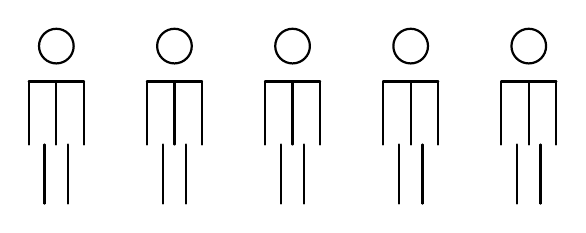
\begin{tikzpicture}[x=1cm,y=1cm,line cap=round,line join=round, thick]
\foreach \x in {0,1.5,3.0,4.5,6.0}{
  \draw (\x,2.0) circle (0.22);
  \draw (\x-0.35,1.55) -- (\x-0.35,0.75);
  \draw (\x+0.35,1.55) -- (\x+0.35,0.75);
  \draw (\x-0.35,1.55) -- (\x+0.35,1.55);
  \draw (\x,1.55) -- (\x,0.75);
  \draw (\x-0.15,0.75) -- (\x-0.15,0.0);
  \draw (\x+0.15,0.75) -- (\x+0.15,0.0);
}
\end{tikzpicture}
\end{figure}

At this opening stage, the five are aggregated visually. But Sandel does not allow them to remain mere units in a sum for very long.

\subsection{Question \& Answer}

\paragraph{Question.} What is morally salient at the start of the case: five separate persons, or one aggregate need of size five?

\paragraph{Answer.} Sandel deliberately makes us keep both descriptions in view. The frame gives us a count, but the speech immediately restores the individuality of the patients by specifying what each of them needs. The lecture begins by aggregating, but only so that it can later test whether that aggregation is morally sufficient.

\section{Five Organs, No Donors}

The next move is to differentiate the five medically while preserving their common urgency. One needs a heart, one a lung, one a kidney, one a liver, and the fifth a pancreas. This slowing-down matters. We are not meant to imagine a mere stack of anonymous claims. We are meant to see five distinct people, each facing death from a different missing organ.

A compact transcript-backed rendering of the setup is
\begin{align}
N_{\text{patients}} &= 5,\\
\text{needed organs} &= \{\text{heart},\ \text{lung},\ \text{kidney},\ \text{liver},\ \text{pancreas}\},\\
N_{\text{donors}} &= 0.
\end{align}
The third line is what turns the medical scene into a moral problem. There are no organ donors. The ordinary path of rescue is closed.

So the first real implication of the case is
\begin{equation}
N_{\text{donors}} = 0
\Longrightarrow
\text{without intervention, the five patients die}.
\end{equation}
Sandel is careful here. He removes the easy alternative before introducing the dangerous one. If there were an available donor pool, there would be no thought experiment. The whole pressure of the case depends on the fact that ordinary medicine has reached its limit.

\section{The Healthy Man in the Next Room}

Only once that scarcity is fixed does the decisive pivot arrive. ``Then it occurs to you'' that in the next room there is a healthy man who came in for a checkup. The transcript becomes noisy for a few seconds around this point, but its stable content is plain enough: one healthy person is nearby, apparently asleep, and his organs could in principle meet the needs of the five.

The new piece of structure is therefore
\begin{equation}
N_{\text{healthy candidates}} = 1.
\end{equation}
This one new datum changes the moral geometry of the case. We are no longer simply facing the tragedy that five people will die. We are facing a proposal.

That proposal is best written without euphemism:
\begin{equation}
\text{save }5\text{ by sacrificing }1.
\end{equation}
Sandel does not yet give us a principle. He gives us an option. And that is important. The case is designed so that the principle will seem to grow out of the scene itself.

\subsection{Question \& Answer}

\paragraph{Question.} Does the appearance of one healthy person convert the case into a permissible trade of one for five?

\paragraph{Answer.} It certainly converts it into a thinkable trade. That is the threshold Sandel wants us to cross. Once the one healthy man is present as a candidate source of organs, the numerical advantage becomes available to thought. Whether it becomes morally available is the question the rest of the case is pressing.

\section{The Arithmetic Under Test}

Now the utilitarian attraction emerges in its simplest form. If what matters is the total number of lives saved, then the comparison appears immediate:
\begin{equation}
5 > 1.
\end{equation}
That inequality is not Sandel's conclusion. It is the temptation the case has been built to generate.

We can make the arithmetic explicit in a way the lecture itself only implies:
\begin{align}
\text{do nothing}
&\Longrightarrow
5 \text{ deaths},\\
\text{kill }1\text{ healthy man and distribute the organs}
&\Longrightarrow
1 \text{ death and }5 \text{ survivals},\\
\Delta N_{\text{lives}}
&=
5 - 1 = 4.
\end{align}
The notation is editorial, but the structure is faithful. If each life is counted symmetrically, the second act seems to improve the total outcome.

That is why the governing rule under examination can be written as
\begin{equation}
\text{maximize lives saved}
\Longrightarrow
\text{kill }1\text{, save }5.
\end{equation}
Again, we should hear this as the candidate rule being tested, not as the settled moral truth of the lecture.

\paragraph{Worked example.} The numerical reasoning proceeds in a few short steps:
\begin{enumerate}
\item There are five patients who will otherwise die.
\item There is one healthy man whose organs could save them.
\item Killing the one would save the five.
\item Therefore a pure maximizing rule points toward sacrificing the one healthy man.
\end{enumerate}
As a piece of counting, this is straightforward. What Sandel is testing is whether moral argument can simply inherit the result of that count.

\subsection{Question \& Answer}

\paragraph{Question.} If the arithmetic points toward killing one to save five, what remains to be argued?

\paragraph{Answer.} Everything turns on whether morality is exhausted by aggregation. Sandel has staged the example so that the arithmetic becomes maximally tempting; the unresolved question is whether the healthy man may be treated as one term in a larger sum, or whether there is a moral barrier that the aggregate gain cannot cross.

\section{Would You Do It?}

Sandel does not conclude this opening movement with a doctrinal statement. He turns back to the room and asks, ``How many would do it?'' This is not merely a classroom flourish. It is the point at which the thought experiment becomes a test of whether we ourselves are willing to inhabit the maximizing logic we have just seen.

The brief laughter in the room matters. It signals that the audience recognizes where the arithmetic is leading, and also that something about the proposed act resists easy endorsement. The lecture now becomes a confrontation between countable gain and moral recoil.

The final fork of the case can be written with complete plainness:
\begin{equation}
\text{kill }1\text{, save }5
\qquad \text{or} \qquad
\text{refuse to kill and let }5\text{ die}.
\end{equation}
That is the power of the example. Both branches are tragic. But only one branch makes the surgeon the intentional killer of an innocent person. Sandel does not yet resolve that tension; he sharpens it by asking who would actually perform the act.

\subsection{Question \& Answer}

\paragraph{Question.} If the count favors one branch, why do so many people still hesitate or refuse?

\paragraph{Answer.} Because the lecture has exposed a gap between numerical superiority and moral permission. Counting seems to support the act. But many listeners recoil from the idea that a surgeon may deliberately kill an innocent patient, even for the sake of producing a better total outcome. The case is designed to bring that gap to the surface.

\section{Summary}

Sandel's transplant-surgeon case is constructed with unusual economy and precision. We begin with another doctor case, then with five patients, then with five different organs, then with the removal of all ordinary donors, then with the single healthy man in the next room, and only then with the proposal to kill one so that five may live. The lecture's mathematical core is simple enough to summarize as
\begin{equation}
\Delta N_{\text{lives}} = 5 - 1 = 4,
\end{equation}
but the point of the lecture is precisely that moral judgment may not be reducible to that expression.

This is what makes the example a serious test of utilitarianism. Sandel lets the maximizing argument appear in its strongest local form and then asks whether we are actually prepared to live by it once the arithmetic has been attached to an intentional human act.